%!TEX root = ../thesis.tex
%*******************************************************************************
%*********************************** First Chapter *****************************
%*******************************************************************************
\chapter{Treatment of uncertainties in computer experiments}
%*******************************************************************************
\hfill
\localtableofcontents
\newpage

%============================================================%
%============================================================%
\section{Introduction}\label{sec:}
%============================================================%
%============================================================%

The progress of computer simulation gradually allows the virtual resolution of more complex problems in scientific fields such as physics, astrophysics, engineering, climatology, chemistry, or biology.
This domain often provides a deterministic solution to complex problems depending on several inputs. 
Associating a UQ analysis with these possibly nonlinear numerical models is a key element to improving the understanding of the phenomena studied. 
A wide panel of UQ methods has been developed over the years to pursue these studies with a reasonable computational cost. 

This chapter presents the standard tools and methods from the generic UQ framework \elias{add ref to intro}, exploited later in this thesis. 
It is structured as follows: Section \elias{add ref} describes the context of the model specification step; 
Section \elias{add ref} presents a classification of the inputs uncertainties and the probabilistic framework to model them; 
Section \elias{add ref} and xx introduce various methods to propagate the input uncertainties through the numerical model for different purposes;
finally, Section \elias{add ref} presents the main inverse methods to perform sensitivity analysis in our framework.


%============================================================%
%============================================================%
\section{Black-box model specification}
%============================================================%
%============================================================%
The uncertainty quantification studies in our framework are performed around an input-output numerical simulation model. 
This numerical model, or code, is hereafter considered as \textit{black-box} since the knowledge of the underlying physics doesn't inform the UQ methods. 
Alternatively, one could consider \textit{intrusive} UQ methods, introducing uncertainties within the resolution of computer simulation (see e.g., \elias{add ref}).
In practice, the numerical model might be a sequence of codes executed in series to obtain a variable of interest.

Moreover, the simulation model is in most cases deterministic, otherwise, it is qualified as intrinsically stochastic (i.e., two runs of the same model taking the same inputs return different outputs).
Then, most numerical simulation presents modeling errors. 
In the following, it will be assumed that the numerical models passed a \textit{validation \& verification} phase, to quantify their confidence and predictive accuracy. 

Formally, part of the problem specification is the definition of the set of $p$ input variables $\bx = \left(x_1, \dots, x_p\right)\TT$ considered uncertain (e.g., wind speed, wave period, etc.). 
In this thesis, the models considered will only present scalar outputs. 
UQ methods dedicated to other types of outputs exist (see e.g., for time series outputs \cite{lataniotis_2019}, \elias{functional Alvaro?}). 
Let us then define the following numerical model:
\begin{equation}
\iM : \bigg|
    \begin{array}{rcl}
        \iD_{\bx} \subseteq \R^p & \longrightarrow & \iD_{\by} \subseteq \R \\
        \bx & \longmapsto & y.
    \end{array}
\end{equation}

Unlike the typical machine learning input-output dataset framework, the UQ analyst can simulate the output image of any inputs (in the input domain), using the numerical model. 
However, numerical simulations often come with an important computational cost. 
Therefore UQ methods should be efficient and require as few simulations as possible. 
In this context, metamodels (or surrogate models) are statistical approximations of the costly numerical model, that can be used to perform tractable UQ. 
Metamodels are only built and validated on a limited number of simulations (in a \textit{supervised learning} framework).
In practice, the model specification step is often associated with the development of a \textit{wrapper} of the code \elias{explain wrapper}, with can be deployed on a \textit{high-perfomance computer}.
Once the model is specified, a critical step of uncertainty quantification is enumerating the input uncertainties and building an associated mathematical model.


%============================================================%
%============================================================%
\section{Enumerating and modeling the uncertain inputs}
%============================================================%
%============================================================%

%------------------------------------------------------------%
\subsection{Sources of the input uncertainties}
%------------------------------------------------------------%

To ensure a complete risk assessment (e.g., associated with the exploitation of a wind turbine throughout its life span), the analyst should construct a list of uncertain inputs as exhaustive as possible. 
Even if these uncertainties might have different origins, they should all be considered jointly in the UQ study. 
The authors proposed to classify them for practical purposes into two groups:
\begin{itemize}
    \item \textbf{aleatory uncertainty} regroups the uncertainties that arise from natural randomness (e.g., \elias{add example}). 
    From a risk management point of view, these uncertainties are qualified as \textit{irreducible} since the industrials facing them will not be able to acquire additional information to reduce them (e.g., additional measures).     
    \item \textbf{epistemic uncertainty} gathers the uncertainties resulting from a lack of knowledge. 
    Contrarily to the aleatory ones, epistemic uncertainties might be reduced by investigating their origin. 
\end{itemize} 

\cite{Kiureghian2009} offers a discussion on the relevance of this classification. 
They affirm that this split is practical for decision-makers to identify possible ways to reduce their uncertainties. 
However, this distinction should not affect the way of modeling or propagating uncertainties. 
\elias{To illustrate the limits of this split, some uncertainties present both an aleatory and epistemic aspect.}
In the following, the probabilistic framework is introduced to deal with uncertainties. 


%------------------------------------------------------------%
\subsection{Modeling uncertain inputs with the probabilistic framework}
%------------------------------------------------------------%

Uncertainties are traditionally modeled with objects from the probability theory.
In this thesis, the \textit{probabilistic framework} is adopted. 
Alternative theories exist to mathematically model uncertainties. 
For example, imprecise probability theory allows more general modeling of the uncertainties. 
It becomes useful when dealing with very limited and possibly contradictory information (e.g., expert elicitation). 
The core probabilistic tools and objects are introduced hereafter. 

The \textit{probability space} (i.e., a measure space with its total measure summing to one), also called probability triple and denoted $(\Omega, \iA, \P)$.
This mathematical concept first includes a sample space $\Omega$, which contains a set of outcomes $\omega \in \Omega$. 
An \textit{event} is defined as a set of outcomes in the sample space.
Then, a $\sigma$-algebra $\iA$ (also called event space) is a set of events. 
Finally, a probability function $\P: \iA \rightarrow [0, 1]$, is a positive probability measure associated with an event.
Most often, the choice of the probability space will not be specified. 
The main object will be functions defined over this probability space: random variables. 

The \textit{random vector} $\bX$ (i.e., multivariate random variable) is a measurable function defined as: 
\begin{equation}
\bX : \bigg|
\begin{array}{rcl}
    \Omega & \longrightarrow & \iD_{\bx} \subseteq \R^p\\
    \omega & \longmapsto & \bX(\omega) = \bx.
\end{array}
\end{equation}
In the following, the random vector $\bX$ will be considered to be a squared-integrable function against the measure $\P$ (i.e., $\int_{\Omega} |\bX(\omega)|^2 \,\d \P(\omega) < \infty$).
Moreover, this work will focus on continuous random variables.

The \textit{probability distribution} of the random vector $\bX$ is the pushforward measure of $\P$ by $\bX$.
Which is a probability measure on $(\iD_{\bx}, \iA)$, denoted $\P_{\bX}$ and defined by: 
\begin{equation}
    \P_{\bX}(B) = \P(\bX \in B) = \P(\omega \in \Omega : \bX(\omega)\in B), \quad \forall B \in \iA.
\end{equation}
The \textit{cumulative distribution function} (CDF) is a common tool to manipulate random variables. 
It is a function $F_{\bX} : \iD_{\bx} \rightarrow [0, 1]$ defined for all $\bx \in \iD_{\bx}$ as: 
\begin{equation}
    F_{\bX}(\bx) = \P(\bX \leq \bx)
            = \P(X_1 \leq x_1, \dots, X_p \leq x_p)
            = \P_{\bX}(]-\infty, x_1] \times \dots \times ]-\infty, x_p]).
\end{equation}
The CDF is a positive, increasing, right-continuous function, which tends to $0$ as $\bx$ tends to $-\infty$ and to $1$ as $\bx$ tends to $+\infty$.
In the continuous case, one can also define a corresponding \textit{probability density function} (PDF) $f_{\bX}: \iD_{\bx} \rightarrow \R_+$  with 
$f_{\bX}(\bx) = \frac{\partial^p F_{\bX}(\bx)}{\partial x_1 \dots \partial x_p}$.

The expected value of a random vector $\E[\bX]$, also called the first moment, is a vector defined as:
\begin{equation}
    \E[\bX] = \int_{\Omega} \bX(\omega) \,\d \P(\omega) =  \int_{\iD_{\bx}} \bx f_{\bX}(\bx) \, \d\bx = \left(\E[X_1], \dots, \E[X_p]\right)\TT.
\end{equation}
In addition, considering two random variables $X_j$ and $X_j$, with $i, j \in \{1, \dots, p\}$, one can write their respective variance:
\begin{equation}
    \var(X_i) = \E\left[X_i - \E[X_i]\right],
\end{equation}
and a covariance describing their joint variability:
\begin{equation}
    \cov(X_i, X_j) = \E\left[\left(X_i - \E[X_i]\right) \left(X_j - \E[X_j]\right)\right].
\end{equation}
The standard deviation $\sigma_{X_j} = \sqrt{\var(X_j)}$ and coefficient of variation $\delta_{X_j} = \frac{\var(X_j)}{|\E[X_j]|}$ are two quantities directly associated to the two first moments.

\elias{Remark on high dimension: We call high dimension anything higher than $p>10$ and it creates issues.}


%------------------------------------------------------------%
\subsection{Joint input probability distribution}
%------------------------------------------------------------%

This section aims at presenting various techniques to model and infer a joint probability distribution (or multivariate distribution).
It will first introduce the \textit{copula}, a universal mathematical tool to model the dependence structure of a joint distribution. 
Then, a few methods to fit a joint distribution over a dataset will be mentioned. 
And finally, a panel of tools to evaluate the goodness of fit between a probabilistic model and a dataset will be recalled. 

From a practical point of view, people tend to properly model the single effects of their input uncertainties. 
However, modeling the dependence structure unlying in a joint distribution is often overlooked.  
To illustrate the importance of this step, \fig{fig:joint_dist_samples} represents three i.i.d samples from three bivariate distributions sharing the same single effects (e.g., here two exponential distributions) but different dependence structures.
One can assume that the joint distribution is the composition of the single effects, also called marginals, and an application governing the dependence between them.
\begin{figure}[ht]
    \centering
    \begin{subfigure}[b]{0.32\textwidth}
        \centering
        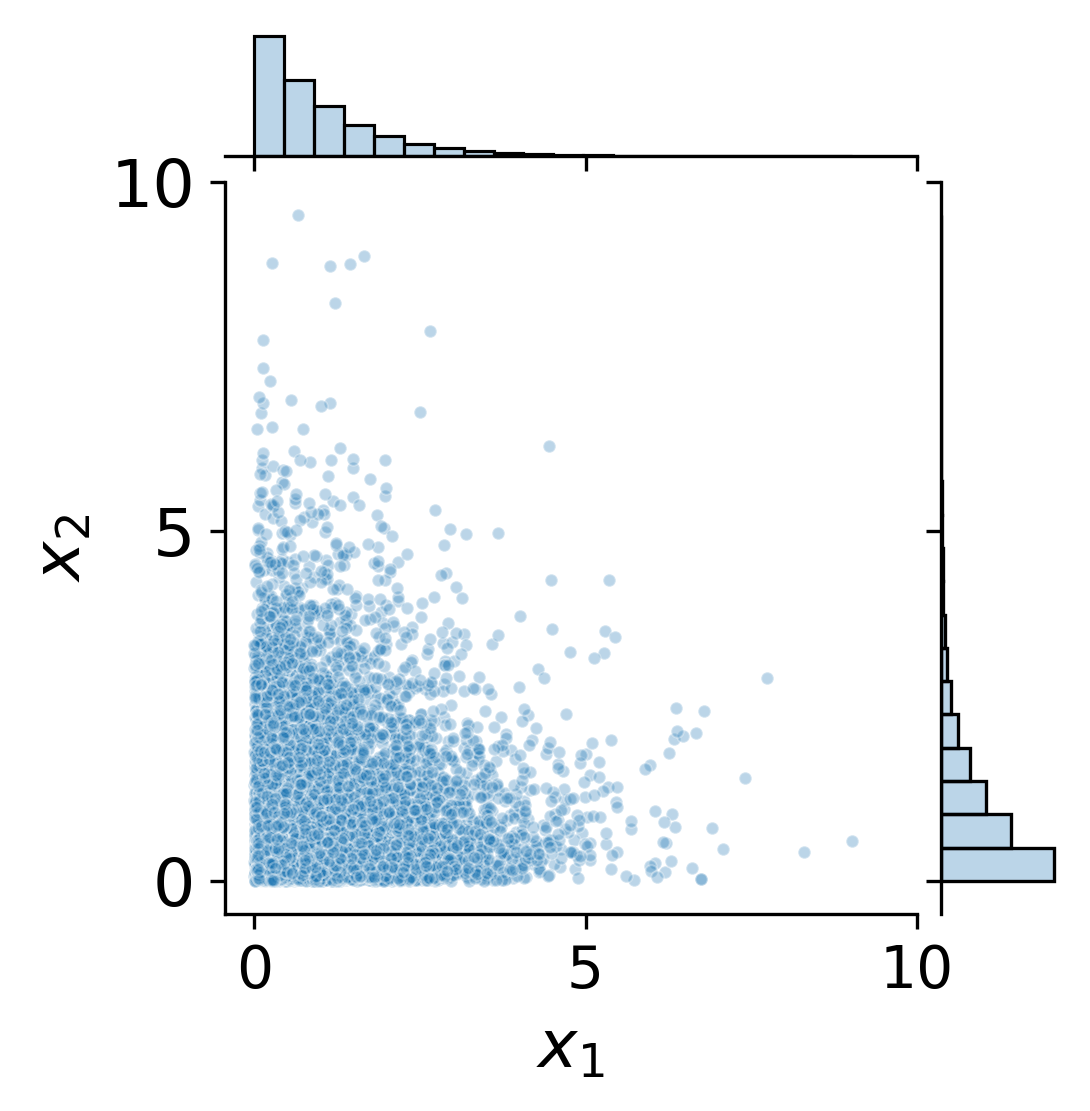
\includegraphics[width=\textwidth]{../numerical_experiments/chapter1/figures/independent_copula.png}
        \caption{Independent copula}
    \end{subfigure}
    \hfill
    \begin{subfigure}[b]{0.32\textwidth}
        \centering
        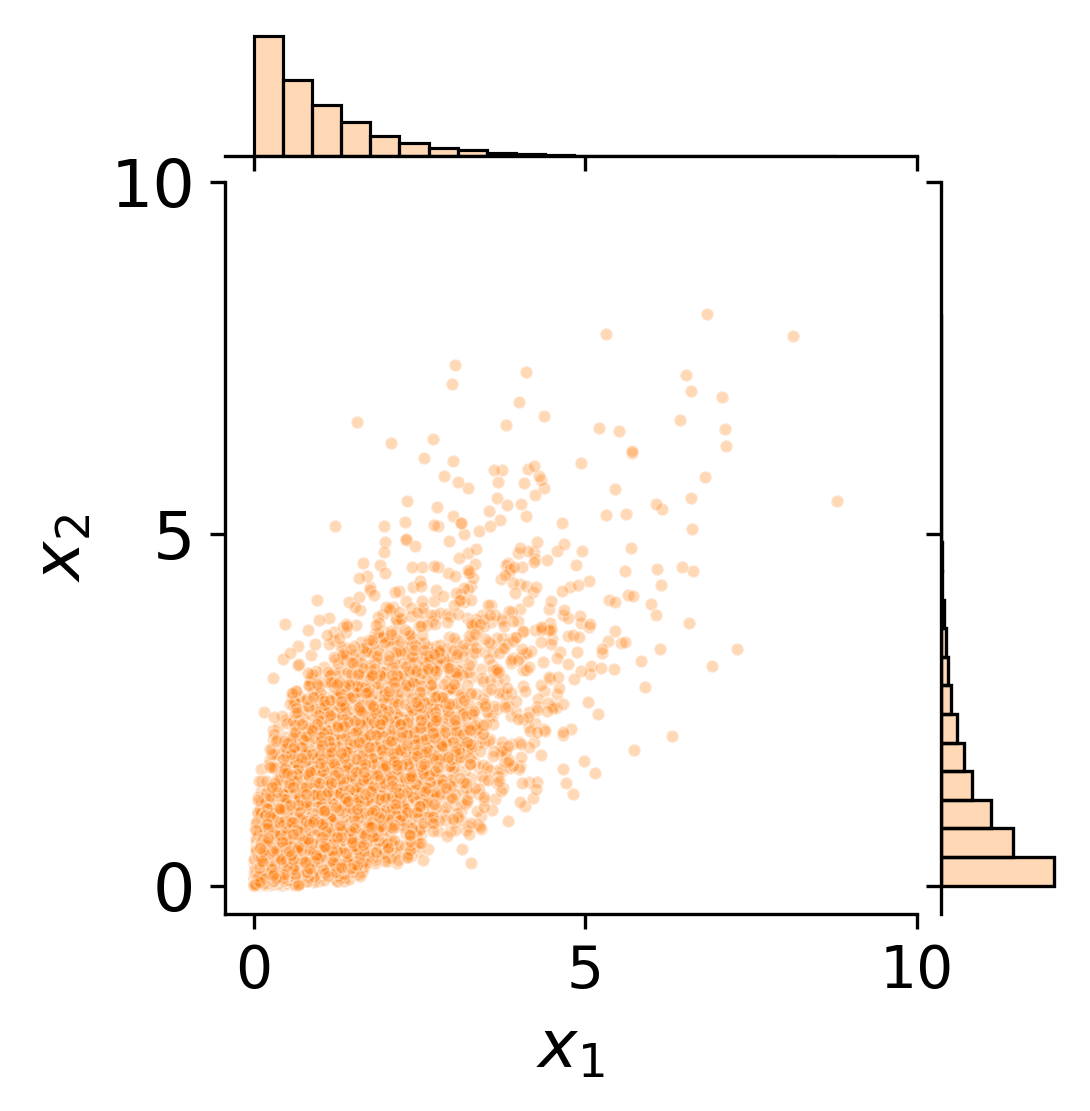
\includegraphics[width=\textwidth]{../numerical_experiments/chapter1/figures/normal_copula.png}
        \caption{Normal copula}
    \end{subfigure}
    \hfill
    \begin{subfigure}[b]{0.32\textwidth}
        \centering
        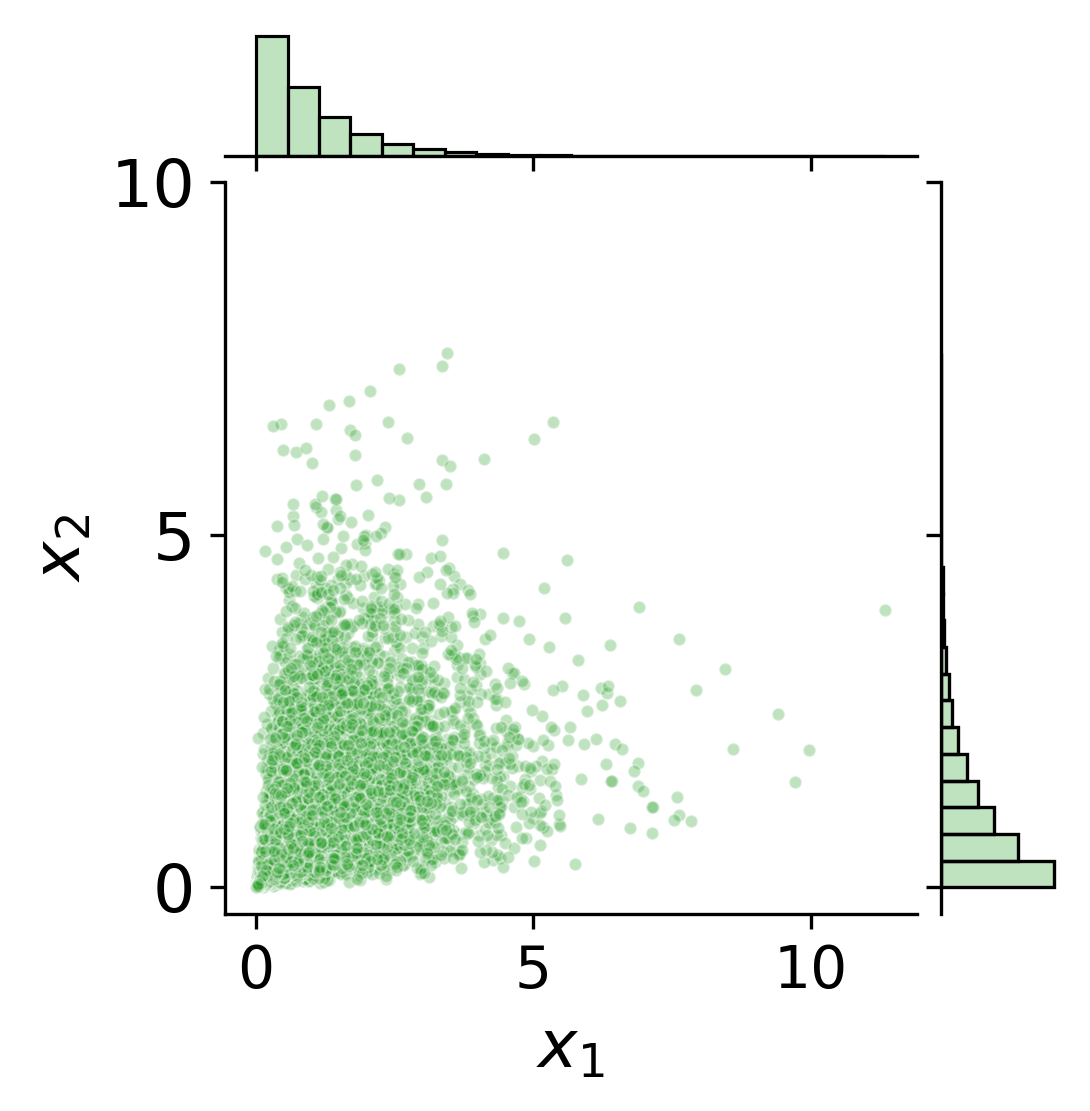
\includegraphics[width=\textwidth]{../numerical_experiments/chapter1/figures/clayton_copula.png}
        \caption{Clayton copula}
    \end{subfigure}
       \caption{Samples of three joint distributions with identical marginals and different dependence structures}
       \label{fig:joint_dist_samples}
\end{figure}

An empirical way of isolating the three dependence structures from this example is to transform the samples in the ranked space. 
Let us consider a $n$-sized sample $\bX_n = \left\{\bx^{(1)}, \dots, \bx^{(n)}\right\} \in \iD_{\bx}^{n}$. 
The corresponding ranked sample is defined as: $\bR_n = \left\{\br^{(1)}, \dots, \br^{(n)}\right\}$, 
where $r^{(l)}_j = \sum_{i=1}^n \1_{\left\{x^{(i)}_j \leq x^{(l)}_j\right\}},$ $\forall j \in \{1, \dots p\}$.
Ranking a multivariate dataset allows us to isolate the dependence structure witnessed empirically. 
\fig{fig:ranked_joint_dist_samples} shows the same three samples from \fig{fig:joint_dist_samples} in the ranked space.
One can first notice that the marginals are uniform since each rank is uniformly distributed. 
Then, the scatter plot from the distribution with independent copula (left plot) is uniform while the two others present different patterns. 
\begin{figure}[ht]
    \centering
    \begin{subfigure}[b]{0.32\textwidth}
        \centering
        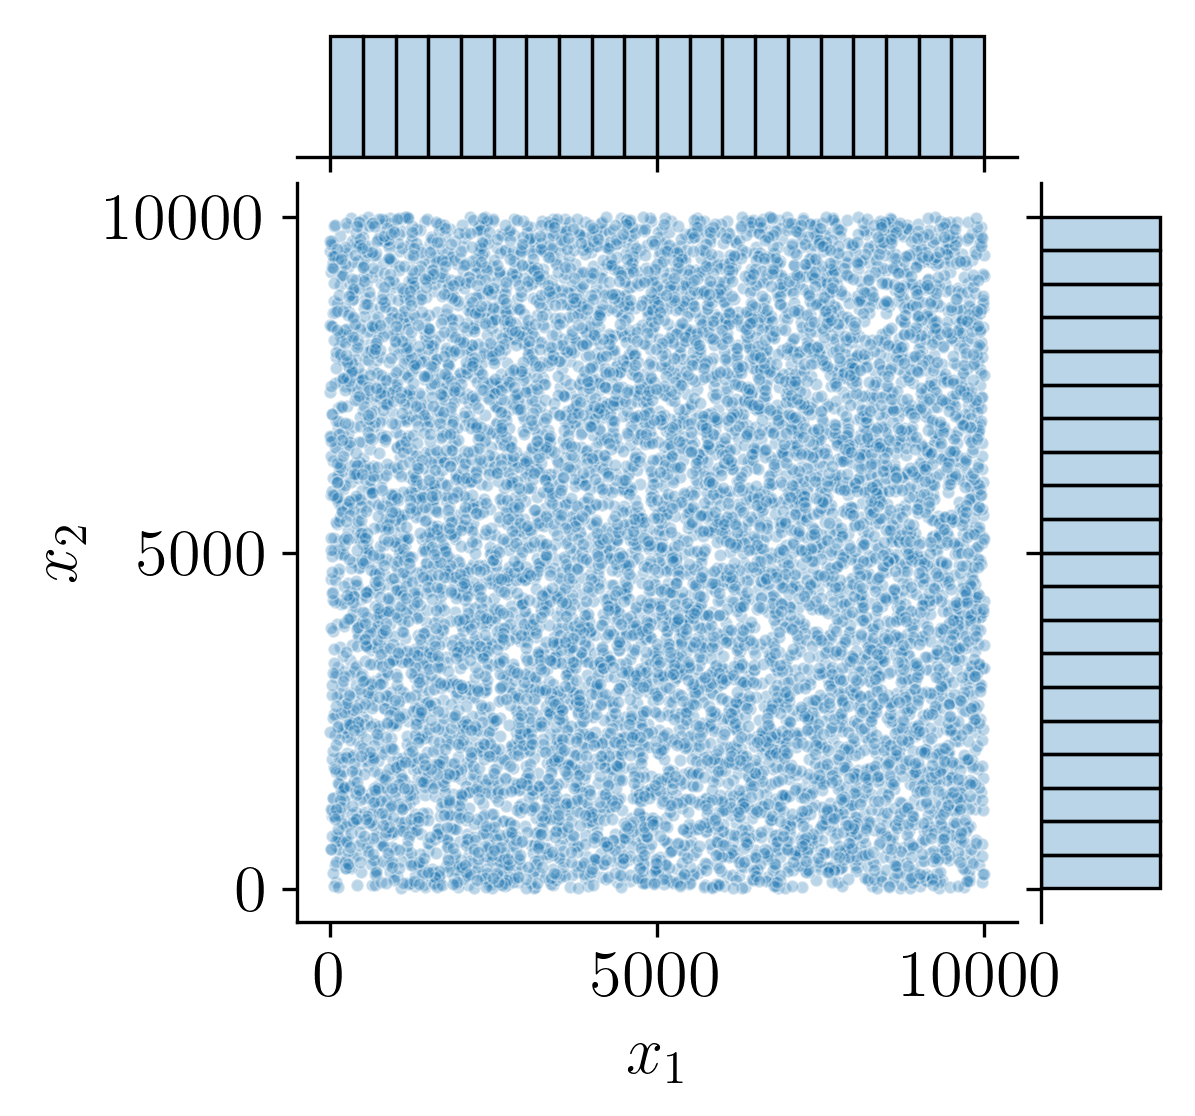
\includegraphics[width=\textwidth]{../numerical_experiments/chapter1/figures/independent_copula_ranked.png}
        \caption{Independent copula}
    \end{subfigure}
    \hfill
    \begin{subfigure}[b]{0.32\textwidth}
        \centering
        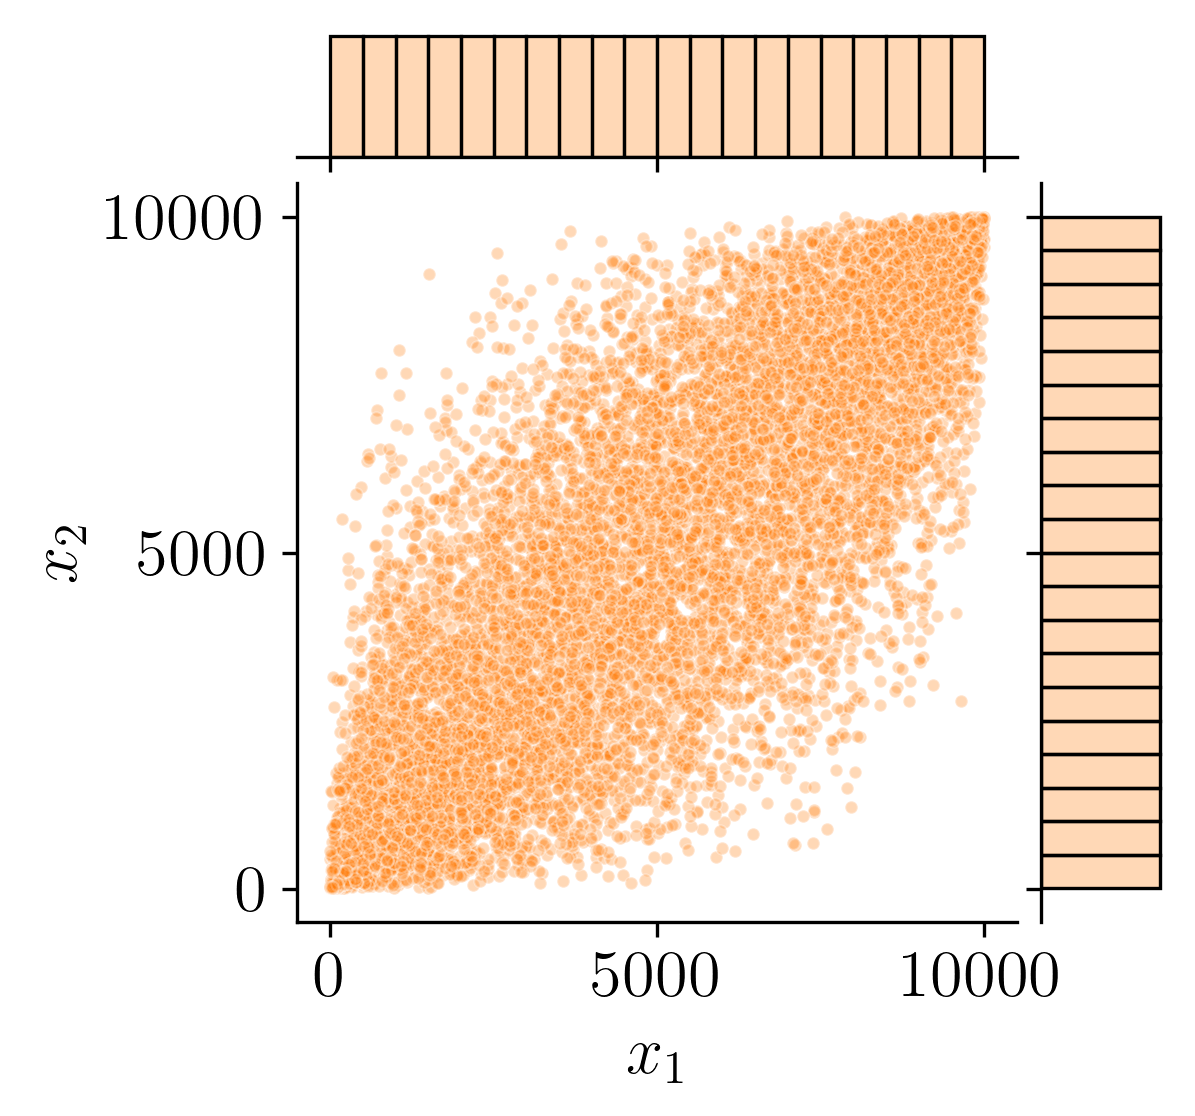
\includegraphics[width=\textwidth]{../numerical_experiments/chapter1/figures/normal_copula_ranked.png}
        \caption{Normal copula}
    \end{subfigure}
    \hfill
    \begin{subfigure}[b]{0.32\textwidth}
        \centering
        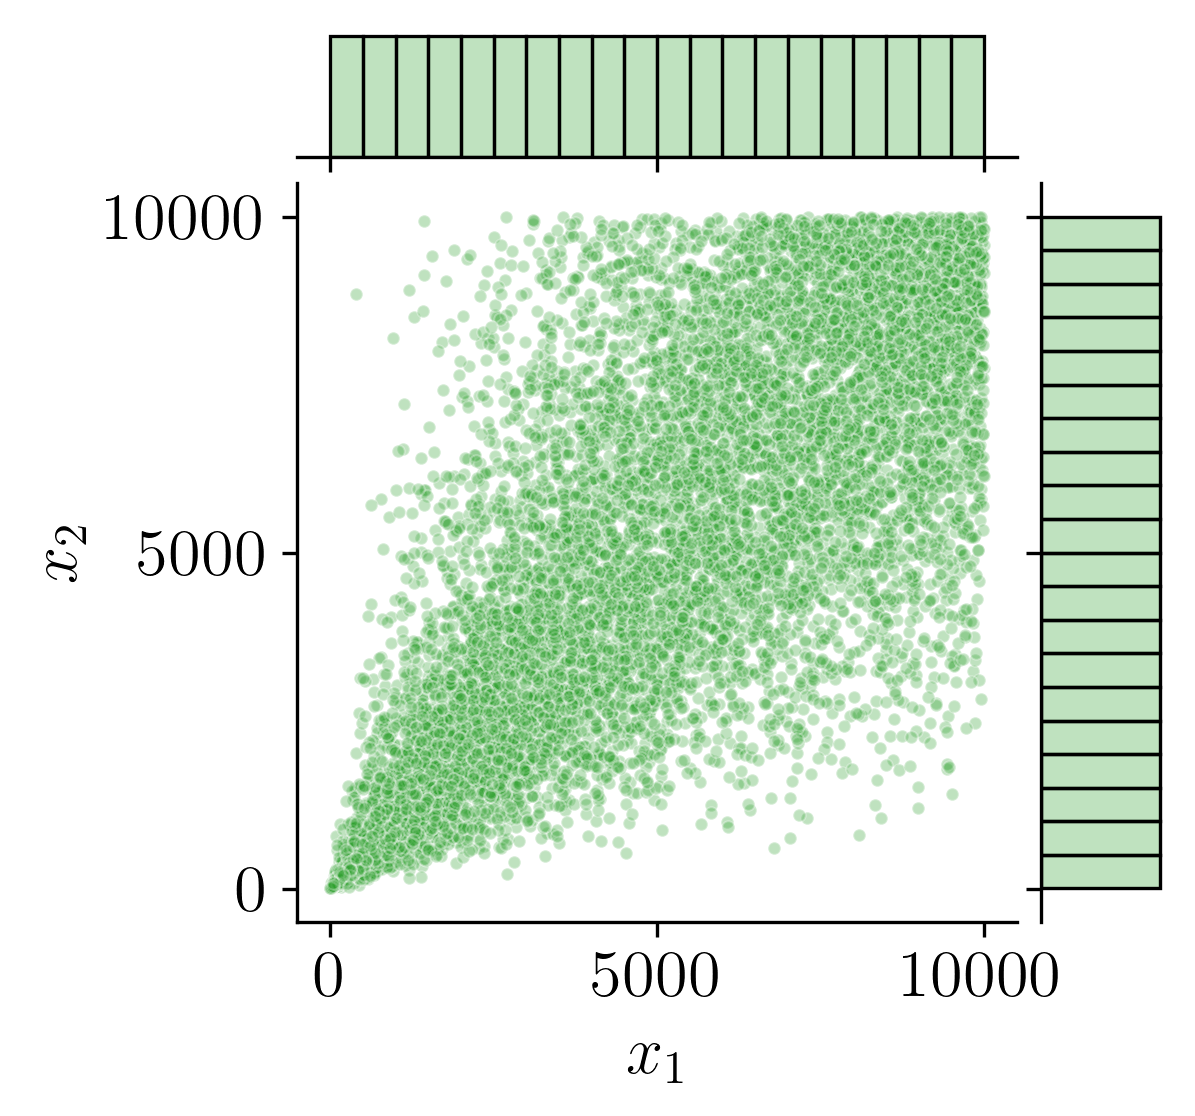
\includegraphics[width=\textwidth]{../numerical_experiments/chapter1/figures/clayton_copula_ranked.png}
        \caption{Clayton copula}
    \end{subfigure}
       \caption{Ranked samples represented in the \fig{fig:joint_dist_samples}}
       \label{fig:ranked_joint_dist_samples}
\end{figure}

A theorem states that the multivariate distribution of any random vector can be broken down into two objects \citep{joe_1997}. 
First, a set of univariate marginal distributions describing the behavior of the individual variables;
Second, a function describing the dependence structure between all variables: a copula. 

\begin{theorem}[Sklar's theorem]
    Let $\mathbf{X} \in \R^p$ be a random vector and its joint CDF $F_{\bX}$ with marginals $\{F_{X_j}\}_{j=1}^p$, there exists a copula $C: [0, 1]^p \rightarrow [0, 1]$, such that:
    \begin{equation}
        F_{\bX}(x_1, \dots, x_p) = C\left(F_{X_1}(x_1), \dots, F_{X_p}(x_p)\right). 
    \end{equation}
    If the marginals $F_{X_i}$ are continuous, then this copula is unique.
    \label{thm:sklar}
\end{theorem}

Theorem \ref{thm:sklar} expresses the joint CDF by combining marginal CDFs and a copula, which is practical for sampling joint distributions. 
Conversely, the copula can be defined by using the joint CDF and the marginal CDFs: 
\begin{equation}
    C(u_1, \dots, u_p) = F_{\bX}(F^{-1}_{X_1}(u_1), \dots, F^{-1}_{X_p}(u_p))
\end{equation}
This equation allows us to extract a copula from a joint distribution by knowing its marginals.
Additionally, copulas are invariant under creasing transformations. 
This property is important to understand the use of rank transformation to display the copula without the marginal effects.     

\elias{define the copula density and address the warning on the confusion.}

Identically to the univariate continuous distributions, a large catalog of families of copulas exists (e.g., independent, Normal, Clayton, Frank, Gumbel copula, etc.).

\elias{define the independent copula, also called product of marginals.}

To infer a joint distribution, this theorem divides the fitting problem into two independent problems: fitting the marginals and fitting the copula
Provided a dataset, this framework allows the combination of a parametric (or nonparametric) fit of marginals with a parametric (or nonparametric) fit of the copula. 

Appendix \ref{apx:A} details the main techniques to estimate marginal distributions. 
Then, Appendix \ref{apx:B} introduces different nonparametric methods to infer a copula, including the empirical Bernstein copula and the Beta copula. 
The adequation between a fitted probabilistic model and a dataset should be validated, therefore, appendices \ref{apx:A} and \ref{apx:B} respectively present visual and quantitative tools for goodness-if-fit evaluation.

To infer a joint distribution over a dataset, the analyst should determine a fitting strategy.
Smart data visualization helps to choose the fitting methods susceptible to be relevant to the problem. 
The following points can be checked at this early stage: 
\begin{itemize}
    \item Is the distribution unimodal? If not, mixtures methods or nonparametric models might be required;
    \item Is the validity domain restrictive? If so, specific families of parametric distributions can be chosen or truncations can be applied;
    \item Is the dimension high? If the dimension is too high: tensorize the distribution as much as possible.
    \item Is the dependence structure complex? Graphically, the dataset in the ranked space gives an empirical description but some independence test exist as well. 
\end{itemize} 



%============================================================%
%============================================================%
\section{Global uncertainty propagation}
%============================================================%
%============================================================%


%============================================================%
\subsection{Numerical integration}
%============================================================%
%------------------------------------------------------------%
\subsubsection{``Good'' properties}
%------------------------------------------------------------%
\elias{Curse of dim / Sequential / Deterministic}

%------------------------------------------------------------%
\subsubsection{Gauss-Kronrod}
%------------------------------------------------------------%

%------------------------------------------------------------%
\subsubsection{Monte Carlo}
%------------------------------------------------------------%

%------------------------------------------------------------%
\subsubsection{Quasi-Monte Carlo and Koksma-Hlawka inequality}
%------------------------------------------------------------%

\subsection{Numerical design of experiments}
%------------------------------------------------------------%
\subsubsection{Space-filling metrics}
%------------------------------------------------------------%
\elias{MinMax / PhiP / MaxMin / Discrepancies}

%------------------------------------------------------------%
\subsubsection{``Good'' properties}
%------------------------------------------------------------%
\elias{Curse of dim / Projections in sub-spaces / Sequential / Deterministic}

%------------------------------------------------------------%
\subsubsection{Monte Carlo and quasi-Monte Carlo designs}
%------------------------------------------------------------%

Monte-Carlo sampling is the simplest way to propagate uncertainty (either for central tendency or probability estimation). 
Using a pseudo-random generator, one can generate $n \in \N$ i.i.d realizations $\left\{\bX^{(i)}\right\}_{i=1,...,n}$ of a random vector $\bX$.

\elias{Remark on randomized quasi-Monte Carlo: paper on quantiles}

%------------------------------------------------------------%
\subsubsection{Latin hypercube sampling}
%------------------------------------------------------------%
The LHS is a method introduced in 1979 \citep{mckay_beckman_1979}, initially created to compute multivariate numerical integrals. 
The main idea is that to make sure that the information is not redundant, the distribution of each sub-projection of the domain should be as uniform as possible. 
To force this concept, each variable's domain is divided into $n$ identical segments creating a square lattice over the domain. 
This lattice is composed of $n^{p}$ squared elements. 
Among the $n^{p}$ elements, the LHS samples $n$ points (only one point by element) with the constraint of having one and only one sample for each segment of each the variables. 
This ensures a good distribution over the sub-projections of the domain. 
Inside each selected element in the square lattice, the points can be placed in the center or randomly.
\elias{Illustration LHS vs. Monte Carlo}

\elias{Illustration pathological LHS (diagonal design)}

%------------------------------------------------------------%
\subsubsection{Optimized latin hypercube sampling}
%------------------------------------------------------------%

\cite{franco_2008} discusses how LHS can have very poor space-filling properties in some cases, which can be prevented by adding an optimization step. 
Knowing that a LHS can be permuted to another one, one can find the permutation on a LHS that would optimize a given space-filling criteria. 
The optimization according to the two following criteria is discussed in \cite{damblin_couplet_2013} and the sub-projections issue is also raised. 
Note that LHS designs are very efficient at exploring a domain but handle poorly some complex dependency models such as copulas.

\elias{Present MaxPro, Uniform Projection designs. The way of optimizing is not the topic. It is more about what are the right criteria}

%============================================================%
\subsection{Central tendency estimation}
%============================================================%
%------------------------------------------------------------%
\subsubsection{Iso-probabilistic transformation}
%------------------------------------------------------------%

%------------------------------------------------------------%
\subsubsection{Central tendency estimation is a probabilistic integration}
%------------------------------------------------------------%



%============================================================%
%============================================================%
\section{Reliability-oriented uncertainty propagation}
%============================================================%
%============================================================%

%============================================================%
\subsection{Problem formalization}
%============================================================%

%------------------------------------------------------------%
\subsubsection{Limit-state function, failure event and domain}
%------------------------------------------------------------%

%------------------------------------------------------------%
\subsubsection{Risk measures \elias{Failure probability, quantile, super-quantile}}
%------------------------------------------------------------%


%============================================================%
\subsection{Rare event estimation methods}
%============================================================%
\elias{Why are the previous sampling methods not suited for rare events?}

%------------------------------------------------------------%
\subsubsection{FORM/SORM}
%------------------------------------------------------------%

%------------------------------------------------------------%
\subsubsection{Monte Carlo}
%------------------------------------------------------------%

%------------------------------------------------------------%
\subsubsection{Importance sampling}
%------------------------------------------------------------%

%------------------------------------------------------------%
\subsubsection{Adaptive sampling (SS/NAIS/IS-CE/Moving particles)}
%------------------------------------------------------------%





%============================================================%
%============================================================%
\section{Sensitivity analysis}
%============================================================%
%============================================================%

%============================================================%
\subsection{Global sensitivity analysis}
%============================================================%

%============================================================%
\subsection{Reliability-oriented sensitivity analysis}
%============================================================%





%============================================================%
%============================================================%
\section{Metamodeling}
%============================================================%
%============================================================%
Note that the calibration error is often larger than the metamodeling error.

%============================================================%
\subsection{Global metamodel}
%============================================================%

%============================================================%
\subsection{Contour finding for rare-event estimation}
%============================================================%






%============================================================%
%============================================================%
\section{Conclusion}
%============================================================%
%============================================================%
